\documentclass[12pt,letterpaper,spanish]{book}

% formato, lenguaje y encoding
\usepackage[utf8]{inputenc}
\usepackage[T1]{fontenc}
\usepackage[spanish, es-nolists, es-lcroman]{babel}
\usepackage[spanish]{babelbib}
\usepackage[top=3cm, left=3cm, bottom=3cm, right=2cm, paper=letterpaper]{geometry}


% Links y numeracion del PDF
\usepackage[pdfpagelabels]{hyperref}

% Codigo Fuente
\usepackage{listings}

% varios
\usepackage{amsmath, amssymb, amsthm}
\usepackage{enumitem} % opciones para itemize 


% ------------- Imágenes -------------------------------------- %
\usepackage[pdftex]{graphicx}	% Para Archivos gráficos         %
\usepackage{float}				% Para usar H!                   %
\usepackage[section]{placeins}	% auto \FloatBarrier por sección %
\usepackage{caption}			% [font=small,labelfont=bf]      %
\usepackage{subcaption}         % Caption para subfiguras        %
\usepackage{sidecap}            % Captions al lado               %
\usepackage{wrapfig}            % Escribir alrededor             %
\graphicspath{{./img/}}         % Agrega Path para buscar imgs.  %
% ------------------------------------------------------------- %

% = = = = = = = = = = = = = = = = = = = = = = =
% TODO NOTES
% = = = = = = = = = = = = = = = = = = = = = = =
\usepackage[pdftex,dvipsnames]{xcolor}  % Coloured text etc.
\usepackage{xargs} % Use more than one optional parameter in a new commands
%\usepackage[colorinlistoftodos,prependcaption,textsize=small]{todonotes}
\usepackage[colorinlistoftodos,prependcaption,textsize=tiny,disable]{todonotes}
\newcommandx{\unsure}[2][1=]{\todo[linecolor=red,backgroundcolor=red!25,bordercolor=red,#1]{#2}}
\newcommandx{\change}[2][1=]{\todo[linecolor=blue,backgroundcolor=blue!25,bordercolor=blue,#1]{#2}}
\newcommandx{\info}[2][1=]{\todo[linecolor=OliveGreen,backgroundcolor=OliveGreen!25,bordercolor=OliveGreen,#1]{#2}}
\newcommandx{\improvement}[2][1=]{\todo[linecolor=Plum,backgroundcolor=Plum!25,bordercolor=Plum,#1]{#2}}
\newcommandx{\thiswillnotshow}[2][1=]{\todo[disable,#1]{#2}}
% = = = = = = = = = = = = = = = = = = = = = = =

\setlength{\parskip}{6pt}


\hypersetup{
    colorlinks,
    linkcolor={black},
    citecolor={blue!50!black},
    urlcolor={blue!80!black}
}


%Para la Carta Gantt
\usepackage{tikz}
\usepackage{gantt}


\begin{document}

%----------------------------------------------------------------------------------------
\begin{titlepage}

\newcommand{\HRule}{\rule{\linewidth}{0.5mm}}

\center % Center everything on the page
 
\ \\[-1cm]

\includegraphics[height=3cm]{./figures/escudoU2014.pdf}\\[0.5cm]
\textsc{\LARGE Universidad de Chile}\\[0cm]
\textsc{\large Departamento de Ingenier\'ia El\'ectrica}\\
\textsc{\large Departamento de Ciencias de la Computaci\'on}\\[3cm]

\HRule \\[0.4cm]
{ \huge \bfseries Dise\~no e Implementaci\'on de Memoria de Largo Plazo para Robots de Servicio}\\[0.1cm] % Title of your document
\HRule \\[0.5cm]

\textsc{\large Propuesta de Memoria para optar al T\'itulo de Ingeniero Civil El\'ectrico e Ingeniero Civil en Computaci\'on.}\\[1cm]

\begin{minipage}{0.4\textwidth}
\begin{flushleft} \large
\emph{Autor:}\\
Mat\'ias \textsc{Pavez}\\
\texttt{\normalsize matias.pavez@ing.uchile.cl} \\
\texttt{\normalsize +569 9888 9358}
\end{flushleft}
\end{minipage}
~
\begin{minipage}{0.4\textwidth}
\begin{flushright} \large
\emph{Profesor Gu\'ia:} (DIE) \\
Javier \textsc{Ruiz del Solar}\\
\texttt{\normalsize jruizd@ing.uchile.cl}
\end{flushright}
\end{minipage}\\[1cm]
\begin{minipage}{0.4\textwidth}
\begin{flushleft}\end{flushleft}
\end{minipage}
~
\begin{minipage}{0.4\textwidth}
\begin{flushright} \large
\emph{Co-Gu\'ia:} (DCC)\\
Jocelyn \textsc{Simmond}\\
\texttt{\normalsize jsimmond@dcc.uchile.cl}
\end{flushright}
\end{minipage}\\[2cm]
{\large Santiago de Chile}\\
{\large Abril, 2017}
\vfill
 
\end{titlepage}
%----------------------------------------------------------------------------------------

% indices
\tableofcontents
%\listoffigures
%\listoftables


\chapter{Introducci\'on}

\section{Antecedentes Generales}

A continuaci\'on se presenta una breve introducci\'on a los temas requeridos para contextualizar este trabajo de t\'itulo: La rob\'otica de servicio y el equipo de trabajo donde se implantar\'a la soluci\'on. Adem\'as, se introduce el tema de la memoria humana, requerido para entender la propuesta y su relaci\'on con la rob\'otica.


\subsection{Robots de servicio}

La rob\'otica de servicio es un \'area enfocada en asistir a los seres humanos en tareas repetitivas y comunes, como la recolecci\'on de basura. Formalmente, se define un \textit{robot de servicio} como un robot ``que realiza tareas \'utiles para humanos o equipamiento, excluyendo aplicaciones de automatizaci\'on industrial''\cite{IFR}. Luego, el robot requiere cierto grado de autonom\'ia, que es la habilidad de actuar a partir del estado actual, usando lo que observa del ambiente y sin intervenci\'on humana. As\'i, un robot de servicio debe trabajar en ambientes no controlados y con la autonom\'ia suficiente que le permita llevar a cabo su cometido.

Un caso de uso t\'ipico es la asistencia en las tareas del hogar, donde se espera que un robot pueda ayudar a ordenar, preparar comida u ofrecer bebestibles. Otros casos de uso consideran el cuidado de adultos mayores, robots para compa\~nia en el hogar, mascotas robots, salud o educaci\'on. Particularmente, la compa\~nia SoftBank Robotics es pionera en ofrecer a Pepper como el primer robot humanoide ya adoptado en hogares de Jap\'on, as\'i como robot de bienvenida en hoteles y tiendas\cite{softbank}.


\subsection{Equipo de Trabajo: UChile Homebreakers}

El laboratorio de rob\'otica del Departamento de Ingenier\'ia El\'ectrica de la Universidad de Chile alberga dos equipos de rob\'otica: \textit{UChile Robotics Team}, dedicado al f\'utbol rob\'otico y \textit{UChile Homebreakers Team}, enfocado en rob\'otica de servicio. Ambos son conformados por alumnos de pregrado y postgrado de diversas especialidades, y liderados por el profesor Javier Ruiz del Solar\cite{uchile-robotics}.

UChile Homebreakers existe desde el a\~no 2007 y actualmente cuenta con 15 estudiantes. Todo su desarrollo de software est\'a basado en ROS, un framework para el desarrollo de plataformas rob\'oticas y con miles de usuarios alrededor del mundo\cite{ROS:2009}.

El equipo trabaja en dos plataformas humanoides, Bender y Pepper. Bender es un robot construido en el mismo laboratorio y con el objetivo de ser un mayordomo para el hogar. Pepper, desarrollado por SoftBank Robotics, est\'a dise\~nado para ser un robot de compa\~nia. Ambos comparten la misma arquitectura de software y pr\'acticamente todo su c\'odigo, exceptuando los drivers para acceder al hardware respectivo.


\subsubsection{RoboCup @Home League}


La RoboCup es una competencia internacional cuyo objetivo es ser un veh\'iculo para el desarrollo de la rob\'otica y la inteligencia artificial. Est\'a compuesta de variadas ligas: Rescue, Soccer, Simulation, @Home, Industrial y Junior, cada una con diversas subligas orientadas a fomentar la investigaci\'on de distintos aspectos del campo. Su sue\~no es que para mediados del siglo 21, un equipo de f\'utbol rob\'otico completamente aut\'onomo sea capaz de vencer al campi\'on de la \'ultima copa mundial y siguiendo las reglas de la FIFA\cite{robocup:rulebook_2017}.

UChile Homebreakers participa desde el a\~no 2007 en la categor\'ia @Home. Las pruebas de la liga se desarrollan en escenarios que imitan ambientes reales, como un hogar o un restaurante. 
%Adem\'as, la competencia funciona como un espect\'aculo para p\'ublico general, por lo que se priorizan pruebas y demostraciones interesantes para los espectadores.
% 
Las capacidades generalmente evaluadas y potenciadas en @Home son de Vision Computacional, Navegaci\'on aut\'onoma, Manipulaci\'on de objetos y Reconocimiento de Voz. Cada a\~no el equipo planifica sus desarrollos de acuerdo a los requerimientos de la competencia, por lo que trabajos fuera de las \'areas mencionadas no son considerados una prioridad.


\subsection{La memoria humana}

La memoria hace relaci\'on al almacenamiento de experiencias en el cerebro. Hay m\'ultiples sistemas de memoria independientes y sustentados por distintas estructuras cerebrales. A grandes rasgos, la memoria se puede dividir en de corto plazo STM (Short-Term Memory) y de largo plazo LTM (Large-Term Memory). La STM maneja informaci\'on muy detallada, es de poca capacidad y permite un r\'apido acceso, mientras que la LTM maneja mucha informaci\'on sobre experiencias y entidades, es menos detallada y de acceso m\'as lento\cite{Eichenbaum:2008}.

La LTM se puede dividir en expl\'icita (consciente) e impl\'icita (inconsciente). La primera almacena datos epis\'odicos, pudiendo responder las preguntas ``Qu\'e'', ``D\'onde'' y ``Cu\'ando'', datos sem\'anticos, que modelan hechos y conceptos como el lenguaje o personas, y tambi\'en, las conexiones entre ambas submemorias. La memoria impl\'icita codifica habilidades, h\'abitos y preferencias.

Existen procesos de consolidaci\'on y deterioro de la memoria que est\'an constantemente en funcionamiento. La consolidaci\'on requiere un est\'imulo relevante, sumado al proceso de almacenamiento, lo que genera conexiones entre la memoria epis\'odica y la respectiva zona sem\'antica. En caso de haber experiencias repetidas, las conexiones se fortalecen. El deterioro de la memoria es un proceso que degenera las conexiones entre ambas formas de memorias expl\'icitas.

La memoria emocional es una forma de memoria impl\'icita que genera reacciones emocionales y sentimientos. Seg\'un los est\'imulos a los que se enfrente, permite modular el proceso de consolidaci\'on de la STM en LTM, modificando el nivel de relevancia de los eventos, pudiendo generar memorias muy fuertes y h\'abitos arraigados. Ejemplos de esto son los flashbacks y las memorias asociadas a eventos importantes.



\section{Motivaci\'on}

La memoria es una habilidad cognitiva crucial para los humanos. Al interactuar con otras personas o el ambiente les permite recordar experiencias pasadas y sus detalles. Luego, es de esperar que un robot de servicio posea una memoria que le permita potenciar sus capacidades de interaci\'on con los humanos que ayudar\'a\cite{Vijayakumar2014}. Una LTM permitir\'ia, por ejemplo, generar di\'alogos interesantes sobre eventos pasados o cosas que el robot puede inferir del comportamiento humano, por otro lado, tambi\'en permitir\'ia la generalizaci\'on de las tareas que tiene que llevar a cabo.

Particularmente, dado el enfoque de las plataformas a utilizar, Bender c\'omo robot mayordomo y Pepper c\'omo robot social, se espera que ambos posean capacidades avanzadas de interaci\'on con los humanos, para lo que se requiere una LTM.


\subsection{Problema}

El a\~no 2015 se desarroll\'o una LTM epis\'odica para el robot Bender, orientada a la interacci\'on con personas y objetos\cite{Sanchez:2015}. El trabajo consideraba m\'etodos para almacenar, adquirir y manejar la informaci\'on epos\'odica, sumado a un proceso simple de consolidaci\'on de memoria.

Actualmente la memoria desarrollada no est\'a operativa, ni es factible habilitarla. A continuaci\'on se listan los aspectos que se consideran causas del problema desde un punto de vista t\'ecnico y humano:
\begin{itemize}
\item No se integr\'o adecuadamente al software del robot, no se recopila ni provee informaci\'on continuamente mientras el robot est\'a en funcionamiento.
\item La memoria no provee una API que siga el est\'andar de los desarrollos del equipo, por lo que no se usa ni es mantenida.
\item RoboCup@Home no considera el uso de LTM en sus competencias, por lo que el equipo no tiene un incentivo real para seguir desarrollando o mantener la memoria. Esto adem\'as ha provocado que el c\'odigo quede obsoleto.
\end{itemize}

Por otro lado, suponiendo que lo anterior estuviese solucionado, a\'un existen los siguientes problemas:
\begin{itemize}
\item S\'olo considera 2 modelos sem\'anticos: Persona y Objeto, para los cuales s\'olo se almacena informaci\'on de nombre, nacionalidad e imagen.
\item A pesar de considerar un modelo para objetos, no se integr\'o con los m\'odulos relacionados que recopilan la informaci\'on, por lo que realmente la memoria s\'olo funciona para entidades de tipo Persona.
\item Es esperable que una memoria considere m\'as modelos (Personas, Objetos, Autos, Ni\~nos, Mascotas, etc) y m\'as caracter\'isticas para cada modelo (nombre, hobbies, trabajo, etc).
\item La consolidaci\'on de memoria STM a LTM s\'olo considera la primera interacci\'on con cada entidad, por lo que no existe actualizaci\'on de los datos.
\item Hay una restricci\'on en los modelos y caracter\'isticas a almacenar, respecto a la informaci\'on que el robot es realmente capaz de obtener.
\end{itemize}


\subsection{Oportunidad}

Existe un vasto desarrollo respecto a la memoria y los procesos cognitivos, sin embargo, la investigaci\'on se concentra en campos como psicolog\'ia, neurolog\'ia y ciencias cognitivas. 
Los estudios de LTM para robots de servicio son muy acotados y no existe una soluci\'on est\'andar a implementar. Algunos robots, como la versi\'on comercial de Pepper, utilizan LTM, pero el c\'odigo asociado no es libre, ni est\'a basado en ROS.

El uso de LTM no est\'a en las prioridades ``RoboCup'' del equipo, sino que es algo \'util para demostraciones y para potenciar la interacci\'on humano-robot. Por ello, se considera que no basta con desarrollar un m\'odulo capaz de recopilar informaci\'on inteligentemente, sino que adem\'as se requiere una integraci\'on con las capacidades de di\'alogo o de inferencia de informaci\'on, para finalmente proveer una demostraci\'on de \'estas habilidades.

As\'i, \'esta es una oportunidad para dise\~nar una LTM para robots de servicio, que considere aspectos como: 
\begin{itemize}
\item Memoria epis\'odica y sem\'antica adecuada a tareas generales de robots de servicio.
\item M\'etodolog\'ia para consolidaci\'on de STM en LTM.
\item Servicio para recopilaci\'on continua de informaci\'on
\item Implementaci\'on est\'andar ROS, adecuada a las plataformas donde se implantar\'a la soluci\'on.
%\item Capacidad de generar respaldos de la memoria y recuperaci\'on de \'estos. 
\item Memoria emocional que permita dar relevancia a los eventos.
\item Inferencia de informaci\'on a partir de datos de la memoria. Por ejemplo: ``Juan suele desayunar a las 9am'', ``El control de la TV suele estar en el sof\'a'', etc.
%\item Integraci\'on con el di\'alogo que realiza el robot.\unsure{quitarlo?}
\end{itemize}

Tanto la memoria emocional, como la inferencia de informaci\'on, se consideran requisitos deseables, por lo que est\'an fuera del \textit{core} del proyecto.

%Tambi\'en se considera que es la oportunidad de promover la inclusi\'on de desafios basados en LTM en la liga @Home, a partir de los resultados de \'este trabajo. As\'i, el desarrollo de LTMs y capacidades asociadas dejar\'ia de ser postergado y pasar\'ia a ser una prioridad para los equipos de la competencia.


%\subsection{Aporte del Trabajo}
%La contribuci\'on del trabajo es principalmente el dise\~no e implementaci\'on 
\todo[inline]{Contribuci\'on del trabajo}

\section{Objetivos}

\subsection{Objetivo General}

El objetivo general corresponde al dise\~no de una LTM para robots de servicio, que considere componentes epis\'odicos y sem\'anticos. La LTM debe ser integrada en Bender y Pepper, con un servicio en background que recopile informaci\'on y con una API acorde a los desarrollos de UChile Homebreakers. Adem\'as, la LTM debe quedar integrada con alguna demostraci\'on de \'esta capacidad, ya sea mediante el di\'alogo o mediante inferencia de informaci\'on.

En resumen, el producto final debe ser una LTM integrada en los robots, de generaci\'on continua de recuerdos y que provea una demostraci\'on de \'esta capacidad.


\subsection{Objetivos Espec\'ificos}

A continuaci\'on se presentan los objetivos espec\'ificos del trabajo, a modo de desglose del objetivo general en tareas m\'as acotadas.

\begin{itemize}
\item Definici\'on del proceso de consolidaci\'on de recuerdos.
\item Dise\~no de la arquitectura del sistema y validaci\'on
\item Implementaci\'on de la LTM y su API.
\item Servicio para recopilaci\'on continua de informaci\'on.
\item Implementaci\'on de la demostraci\'on.
\end{itemize}

Otros objetivos espec\'ificos, correspondientes a requisitos que no son del \textit{core} del proyecto, son la implementaci\'on de la memoria emocional y la implementaci\'on de un m\'odulo de inferencia de informaci\'on basada en LTM.


%\section{Alcances}
\todo[inline]{ALCANCES}

%\section{Estructura de la memoria}
\todo[inline]{ESTRUCTURA DE LA MEMORIA1}


\chapter{Contextualizaci\'on}

\todo[inline]{INTRO AL CAPITULO!, explicando los temas variados!}

% ================================================================
% ================================================================
% ================================================================

\section{Robots de servicio}

La Federaci\'on Internacional de Rob\'otica (IFR)\cite{IFR} define \textit{robot} como:
\begin{quotation}
``Un mecanismo actuado y programable en dos o m\'as ejes y con un cierto grado de autonom\'ia, que se mueve en su entorno para realizar tareas previstas. En este contexto, autonom\'ia se refiere a la habilidad de realizar tareas previstas, basado en el estado actual y lo sensado, sin intervenci\'on humana.''
\end{quotation}

Asimismo, la IFR define un \textit{robot de servicio} como un robot ``que realiza tareas \'utiles para humanos o equipamiento, excluyendo aplicaciones de automatizaci\'on industrial''. As\'i, un robot de servicio debe trabajar en ambientes no controlados y con la autonom\'ia suficiente que le permita llevar a cabo su cometido. Generalmente, la rob\'otica de servicio se enfoca en asistir a los seres humanos en tareas repetitivas y comunes.

Seg\'un su \'area de aplicaci\'on, un rob\'ot de servicio se clasifica en \textit{de uso personal} o \textit{de uso profesional}. Los primeros son utilizados en ambientes no comerciales y por personas comunes; como por ejemplo, un robot sirviente o una silla de ruedas aut\'onoma. Un robot de servicio profesional se utiliza en ambientes comerciales, usualmente operados por alguien entrenado; un ejemplo son los robots de entrega de paquetes o para cirug\'ia.


\subsection{Robots Dom\'esticos}

Seg\'un la recopilaci\'on de datos realizada por la IFR durante el 2016, este tipo de robots es utilizado en las siguientes \'areas:
\begin{itemize}[topsep=0pt]
\setlength\itemsep{0.2em}
\item Tareas dom\'esticas: De compa\~nia, asistencia, limpieza, cuidado del hogar.
\item Entretenimiento: Juguetes, comunicaci\'on, educaci\'on e investigaci\'on.
\item Asistencia a ancianos y discapacitados: Sillas rob\'oticas y robots para cuidar personas.
\item Transporte.
\item Seguridad y vigilancia.
\item Otros que no caen en las categor\'ias anteriores.
\end{itemize}
\bigskip

El foco de este trabajo son los robots de servicio personales, dedicados a tareas dom\'esticas, clasificaci\'on a la que en  adelante se referir\'a como \textit{Robots Dom\'esticos}.

Para entender el alcance del trabajo, en cuanto a qu\'e es lo que se espera del sistema, a continuaci\'on se listan algunas capacidades de los robots dom\'esticos. Un robot de compa\~nia y asistencia tiene, pero no se limita a las siguientes tareas:
\begin{itemize}[topsep=0pt]
\setlength\itemsep{0.2em}
\item Interacci\'on amistosa con humanos.
\item Ayudar a recordar y organizar tareas.
\item Cooperar con la realizaci\'on de un procedimiento.
\item Guiar y seguir a personas.
\item Recordar informaci\'on y entidades.
\end{itemize}
\bigskip

Algunas tareas que robots dom\'esticos de tipo mayordomo deben ejecutar son:
\begin{itemize}[topsep=0pt]
\setlength\itemsep{0.2em}
\item Ofrecer comida y bebestibles.
\item Preparaci\'on de comida.
\item Ordenar y limpiar el hogar.
\end{itemize}
\bigskip

% ================================================================
% ================================================================
% ================================================================

\section{Memoria Humana}

\todo[inline]{Faltan varias referencias!... ver... referencias a psicoanalisis \cite{Deutsch2008} }


La memoria es un elemento fundamental para los humanos en su d\'ia a d\'ia, es parte integral de su existencia. P ermite recordar qui\'en, qu\'e, c\'omo, d\'onde y cu\'ando. En t\'erminos psicol\'ogicos, es la habilidad para para codificar, almacenar y luego obtener informaci\'on sobre eventos pasados, en el cerebro. Los pensamientos son parte de la memoria de corto plazo, mientras que eventos pasados son almacenados en una memoria de largo plazo. Existen muchos estudios en el \'area de la psicolog\'ia cognitiva con diversas descripciones y modelos te\'oricos de cada tipo de memoria\cite{Vijayakumar2014}.

Desde el punto de vista de la informaci\'on procesada, la memoria es vista como una facultad humana consistente en procesos para el manejo de informaci\'on. Los 3 componentes principales son:

\begin{itemize}
\item Codificaci\'on: En este paso, se adquiere nueva informaci\'on desde los sentidos humanos. Los datos son convertidos a un formato que pueda ser almacenado en la estructura cerebral correspondiente.
\item Almacenamiento: Consiste en la creaci\'on de registros permanentes de informaci\'on. Es un proceso pasivo, de continuo procesamiento para clasificar datos nuevos y los ya existentes en el cerebro.
\item Adquisici\'on: Hace referencia al acceso de datos almacenados. El proceso se realiza en el momento, para obtener una reconstrucci\'on aproximada de la informaci\'on, a partir de elementos repartidos en distintas partes del cerebro.
\end{itemize}


La memoria puede ser dividida en m\'ultiples sistemas de independientes, con funcionalidades bien definidas y sustentados por distintas estructuras cerebrales. La primera diferenciaci\'on define dos tipos de memoria: la memoria de corto y la de largo plazo, STM (Short-Term Memory) y LTM (Long-Term Memory), por sus siglas en ingl\'es. En el diagrama de la figura \ref{img:human_memory} se muestra una separaci\'on cl\'asica utilizada en el \'area de las ciencias cognitivas\cite{Eichenbaum:2008}, explicada en las siguientes subsecciones.

\begin{figure}[H]
\centering
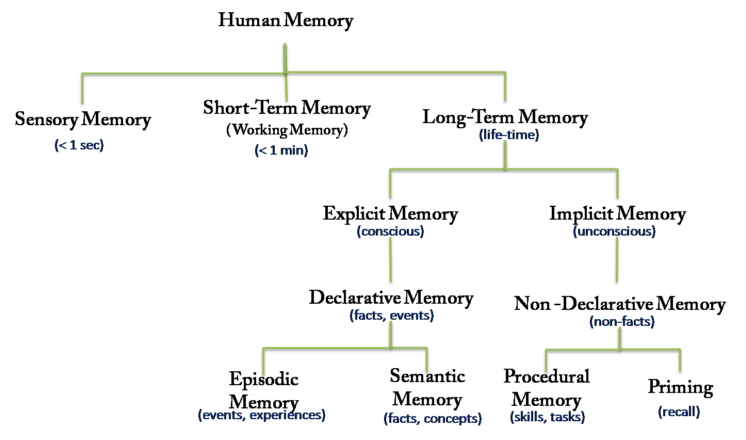
\includegraphics[width=0.8\textwidth]{./figures/diagrama_memoria.png}
\caption{\small Clasificaciones de la memoria humana. Obtenido de \cite{Vijayakumar2014}.}
\label{img:human_memory}
\end{figure}

% Sobre el estudio de la memoria.. origenes.. Tulving 

\subsection{Memoria de Corto Plazo}

En el \'ambito cognitivo, la STM se refiere a la habilidad de estar atento, recopilar informaci\'on  y memorias, para luego utilizarlas dentro de un corto periodo de tiempo. Es responsable de almacenar informaci\'on constantemente y de decidir que parte ser\'a transferida a la memoria de largo plazo. El t\'ermino de \textit{Memoria de Trabajo} suele ser utilizado de manera intercambiable con el de STM. Adem\'as, suele ser agrupada con otro tipo de memoria, llamada \textit{Sensorial}.

La STM se caracteriza por manejar informaci\'on muy detallada, ser de poca capacidad y permitir un r\'apido acceso a estos datos. Permite recordar r\'apidamente y con gran detalle experiencias ocurridas hace pocos segundos, pero con dificultad creciente a medida que avanza el tiempo.

Se sustenta principalmente en la corteza prefrontal del cerebro. Algunos estudios han mostrado que las neuronas involucradas son capaces de mantener informaci\'on relevante de corto plazo, la que es combinada con informaci\'on sensorial entrante y \'areas que manejan la toma de decisiones. %(Miller, 2000).
En los humanos esta \'area presenta gran activaci\'on durante procesos de codificaci\'on, acceso y manipulaci\'on de memorias. %(Postle, 2006). 


\subsection{Memoria de Largo Plazo}

La LTM se asocia al almacenamiento permanente de informaci\'on en el cerebro. Se caracteriza por manejar mucha informaci\'on sobre experiencias y entidades, ser menos detallada y proveer un acceso m\'as lento a los recuerdos, respecto a la STM\cite{Eichenbaum:2008}. Cierta informaci\'on de la STM eventualmente es transferida a la LTM. De acuerdo a la figura \ref{img:human_memory}, sus dos principales categor\'ias son la \textit{Memoria Impl\'icita} y la \textit{Memoria Expl\'icita}.
% algunos creen que no est\'a limitada en su capacidad de almacenar informaci\'on.

\subsubsection{Memoria Impl\'icita}

La memoria impl\'icita  abarca la capacidad de aprender habilidades, h\'abitos y preferencias, caracterizados por ser mejorados o adquiridos sin una recolecci\'on consciente. As\'i, tambi\'en suele ser denominada \textit{memoria inconsciente} o \textit{memoria no declarativa}, pues comprende acciones que pueden ser realizadas sin pensar en ellas. Ejemplos de esto, son el andar en bicicleta o tocar un instrumento musical.

Se puede clasificar en \textit{memoria procedural} (P-LTM) y en \textit{memoria de primado}. La primera ayuda a realizar tareas sin pensar en ellas, es decir, maneja el conocimiento del \textit{C\'omo}; Ejemplos de esto son comer y caminar. La memoria de primado hace referencia a la predisposici\'on para recordar hechos o informaci\'on a la que un sujeto es expuesto con anterioridad; Ejemplos de esto son la facilidad para recordar canciones escuchadas hace poco tiempo, o el uso de palabras e ideas vistas recientemente.

Se ha mostrado que la P-LTM se sustenta en el cerebelo, mediante la activaci\'on de este durante el uso de habilidades motoras.

Otro tipo de memoria implic\'ita es la \textit{memoria emocional} (Em-LTM). Se encarga de dar significado afectivo a ciertos  est\'imulos, que de otra forma ser\'ian neutrales. Las estructuras cerebrales involucradas son la am\'igdala, \'areas corticales y subcorticales. Esta memoria se expresa mediante la activaci\'on del hipot\'alamo, en conjunto al sistema nervioso simp\'atico, generando reacciones emocionales y sentimientos.


\subsubsection{Memoria Expl\'icita}

La memoria expl\'icita suele ser denominada \textit{memoria consciente} o \textit{memoria declarativa}, pues maneja conocimientos relacionados a hechos y eventos adquiridos de forma consciente. Seg\'un las estructuras cerebrales involucradas, se conforma de la \textit{memoria epis\'odica} y de la \textit{memoria sem\'antica}.

La memoria epis\'odica (Ep-LTM) es de car\'acter  autobiogr\'afico y almacena detalles de eventos y experiencias pasadas. Permite responder a las preguntas ``Qu\'e sucedi\'o'', ``D\'onde ocurri\'o'' y ``Cu\'ando ocurri\'o''. Un humano puede acceder a esta memoria si es capaz de decir: ``recuerdo que''. Este tipo de memoria da al ser humano la sensaci\'on de continuidad en el tiempo.

La memoria sem\'antica (S-LTM) almacena el conocimiento de hechos, significados, categor\'ias y proposiciones. Un humano puede acceder a esta memoria si es capaz de decir: ``s\'e que''. Esta memoria se abstrae de perspectiva e informaci\'on situacional.

Las estructuras cerebrales que soportan la memoria expl\'icita son el hipocampo, encargado de manejar la Ep-LTM, junto a la corteza cerebral, en donde se distribuyen los conocimientos de la S-LTM. En el hipocampo se mantienen conexiones neuronales a los sectores de inter\'es de la corteza, en donde se alojan conocimientos sem\'anticos asociados a cada episodio.

Un ejemplo de uso de Ep-LTM es el recuerdo de una graduaci\'on escolar, el lugar y la fecha donde ocurri\'o. La S-LTM podr\'ia responder en que consiste una graduaci\'on y describir la ropa que se suele ocupar en ellas.


\subsection{Plasticidad Sin\'aptica y Modulaci\'on}

Se denomina \textit{consolidaci\'on} de memoria al proceso de transici\'on de conocimiento desde la STM a la LTM. Durante la consolidaci\'on se generan conexiones neuronales entre la Ep-LTM y la respectiva zona sem\'antica. Para activar la consolidaci\'on se requiere de un est\'imulo relevante, sumado a la cadena de eventos para el almacenamiento.

Se denomina \textit{deterioro} de memoria u ``olvido'' al proceso de debilitamiento de las conexiones neuronales establecidas por los procesos de consolidaci\'on. Est\'a en constante funcionamiento, degenerando las asociaciones entre la Ep-LTM y la S-LTM. Por lo tanto, en este contexto, el olvido no significa una eliminaci\'on de los datos en el cerebro, sino que estos siguen ah\'i, pero la conexi\'on requerida es inexistente o es demasiado d\'ebil para poder ocuparla.

Existen procesos qu\'imicos a nivel cerebral que afectan la consolidaci\'on y el deterioro de la LTM. Hay evidencia de que estos est\'an en continuo funcionamiento. Estos eventos celulares ocurren en una escala de segundos a minutos, y son esenciales para la mantenci\'on de la memoria a largo plazo.

Es posible modular ambos procesos. Las experiencias repetidas potencian la consolidaci\'on de la memoria, lo que fortalece las conexiones neuronales. Por otro lado, la memoria emocional es capaz de potenciar o deprimir las reacciones qu\'imicas requeridas; seg\'un los est\'imulos a los que se enfrente, modifica el nivel de relevancia de los eventos, pudiendo generar memorias muy fuertes y h\'abitos arraigados. Ejemplos de esto, son la memorizaci\'on por repetici\'on, los flashbacks y las memorias asociadas a eventos importantes como cumplea\~nos.

% ================================================================
% ================================================================
% ================================================================

\section{Memoria y rob\'otica}

En esta secci\'on se presenta el estado del arte respecto al uso de LTM en rob\'otica. En primer lugar se presenta la importancia de la LTM y las expectativas para un robot dom\'estico. Luego se hace una comparaci\'on entre la memoria humana y el manejo de informaci\'on en robots.  Se presenta el estado del arte para cada componente cognitivo de inter\'es. Finalmente, se describen otros enfoques de la literatura para la implementaci\'on de LTMs, que no est\'an basados en el enfoque biol\'ogico utilizado en este proyecto.


\subsection{Relevancia de la memoria rob\'otica}

La memoria es una habilidad esencial para cualquier ser social. Lo mismo aplica para un robot dom\'estico cuya misi\'on sea establecer una relaci\'on de largo plazo con usuarios humanos. Un problema com\'un es que los usuarios tienden a perder el inter\'es r\'apidamente en los robots, debido a la falta de vida y expectativas no cumplidas, respecto a la inteligencia y capacidad de socializar de la m\'aquina. El problema se potencia con el paso del tiempo, donde la motivaci\'on por interactuar disminuye y se genera frustraci\'on, a medida que el robot continua repitiendo los mismos comportamientos predefinidos\cite{Ho2009}.

Si se desea mejorar la interacci\'on humano-robot, entonces se requiere que el robot se comporte de manera m\'as natural. Los mejores agentes rob\'oticos sociales deber\'ian satisfacer las necesidades cognitivas y sociales humanas; mientras m\'as familiar sea la interacci\'on, ser\'an m\'as efectivos en su prop\'osito. As\'i, la LTM es una habilidad crucial si se espera que el robot sea capaz de aprender y adaptarse a su entorno.


Por otro lado, desde un punto de vista pr\'actico, se ha mostrado que el concepto de memoria LTM aplicada a robots es beneficioso. En \cite{Salgado2012} ocupan memoria P-LTM para mejorar el desempe\~no de un robot en ambientes din\'amicos, logrando acelerar el proceso de adaptaci\'on al entorno y la toma de decisiones.

%... blabla util \cite{Vijayakumar2014}


%\subsubsection{Requerimientos para robots dom\'esticos}
%
%En t\'erminos de LTM, un robot dom\'estico necesita poder recordar los siguientes conocimientos:
%
%... \todo[inline]{tareas de un robot de servicio}
%\begin{itemize}
%\item 
%\end{itemize}
%
%... casos de uso e inferencia \cite{Vijayakumar2014}
%
%... artificial companion PAG 13 \cite{Vijayakumar2014}
%


\subsection{Relaci\'on entre memoria humana y memoria rob\'otica}


Son muchos los trabajos en LTM que han basado su desarrollo en la taxonom\'ia de la memoria humana, donde se implementan esquemas de informaci\'on con m\'odulos an\'alogos a los presentados en la figura \ref{img:human_memory}. Esto se puede justificar por la similitud de cada tipo de memoria, con m\'odulos preexistentes en la arquitectura rob\'otica. A continuaci\'on se presenta una comparaci\'on entre cada tipo de memoria y sus procesos, y el an\'alogo rob\'otico.

\subsubsection{Memoria STM}

Se relaciona a todos los datos que est\'an actualmente cargados en la memoria primaria de la m\'aquina. Esta memoria es la utilizada para solucionar la tarea actual, es equivalente a los pensamientos del robot y cumple con las caracter\'isticas de la STM humana: es volátil, de r\'apido acceso y limitada en capacidad. Tambi\'en se encuentra presente en todo archivo temporal manejado por el sistema, mientras est\'a en funcionamiento. As\'i, la estructura equivalente a la cerebral ser\'ia la RAM de la m\'aquina.


\subsubsection{Memoria S-LTM}

La memoria S-LTM es com\'un y se puede asociar a casi toda fuente de datos est\'atica, no utilizada por las otras memorias. Luego, la S-LTM se sustenta en la memoria secundaria, cumpliendo las caracter\'isticas de la LTM humana: es persistente, de acceso costoso y virtualmente ilimitada en capacidad. Algunos ejemplos son:
\begin{itemize}[topsep=0pt]
\setlength\itemsep{0.2em}
\item Bases de datos.
\item Directorios con im\'agenes de personas y objetos conocidos.
\item Mapa con descripci\'on del ambiente.
\item Frases predefinidas que puede decir el robot.
\item Archivos de audio utilizados por el robot.
\item En general, todo archivo con datos persistentes, cargados en cada sesi\'on de trabajo.
\end{itemize}


\subsubsection{Memoria P-LTM}

Este tipo de memoria es comparable a algoritmos predefinidos para realizar acciones, generalmente motoras. 

Algunos ejemplos comparables son: 
\begin{itemize}[topsep=0pt]
\setlength\itemsep{0.2em}
\item Algoritmos basados en redes neuronales, entrenados para manipular objetos o reconocer patrones.
\item Algoritmos entrenados para tareas espec\'ificas, c\'omo la detecci\'on de caras o el reconocimiento de voz.
\item Controladores basados en puntos de operaci\'on para acciones motoras.
\item S\'intesis de voz
\end{itemize}

Las estructuras equivalentes a la versi\'on cerebral ser\'ian los archivos con par\'ametros para cada algoritmo, obtenidos a partir del entrenamiento o ajustados manualmente.


\subsubsection{Otros tipos de memoria}

Generalmente, tanto STM, S-LTM como P-LTM son un requisito m\'inimo para el funcionamiento de un software rob\'otico, por lo que no son implementadas conscientemente. Luego, la existencia de tales memorias, no implica la intenci\'on de crear una arquitectura LTM similar a la humana. Los otros tipos de memorias s\'olo son implementados en casos especializados.



\subsection{Memoria LTM expl\'icita}\label{sec:ltm_exp}

%Han existido diversos intentos por crear memorias epis\'odicas y sem\'anticas. ... tal persona hizo tal cosa ....

No existe un consenso sobre los contenidos, el formato o las herramientas para implementar Ep-LTM.
%... que recordar y cuando \cite{Kasap2010}
%... modelo de contexto \cite{Sanchez:2015} FELIX

% ... Considerar unificaci\'on de informaci\'on.. que pasa si almaceno obj1 y obj2, pero luego aprendo que son el mismo?
%...... S Memory.. se abstrae de perspecttiva y cosas situacionales \cite{Stachowicz2012}

Sin embargo, si existe una aceptaci\'on generalizada sobre los requerimientos m\'inimos y deseables para el dise\~no\cite{Vijayakumar2014}\cite{Ho2009}\cite{Stachowicz2012}\cite{Jockel2008}:

\subsubsection{Aspectos de dise\~no m\'inimos}

% Stachowicz2012
% The first three requirements are given by the criteria of Clayton et al [14]

% corregirlos

\begin{enumerate}[topsep=0pt]
\setlength\itemsep{0.2em}
\item Contenido: (R1) Informaci\'on de eventos pasados debe ser recolectada e indexada respecto a su contexto espacio-temporal: Qu\'e, d\'onde y cu\'ando pas\'o.

\item Estructura: (R2) Cada evento en conjunto con su contexto espacio-temporal forman una \'unica representaci\'on integrada, que debe ser recordada como un todo, en caso de obtener cualquiera de las caracter\'isticas del evento.

\item Flexibilidad: (R3) La informaci\'on almacenada es declarativa por naturaleza, y puede ser flexiblemente almacenada. Particularmente, puede interactuar con conocimiento sem\'antico, incluso si este fue obtenido con posterioridad a la codificaci\'on del episodio.

\item Datos espec\'ificos: (R4) Memoria epis\'odica cuenta con s\'olo una instancia de cada evento para su entrenamiento, pues cada evento tiene caracter\'isticas espec\'ificas a la situaci\'on.

\item Ep-LTM es LTM y declarativa: (R5) La memoria epis\'odica es una forma de memoria LTM. Puede almacenar recuerdos por segundos, minutos, d\'ias o a\~nos. Tambi\'en es una forma de memoria declarativa.

\item Perspectiva: (R6) Memoria epis\'odica debe lidiar con datos espec\'ificos al evento, lo que implica una perspectiva. Es decir, eventos recordados deben mantener la misma perspectiva que se ten\'ia en la experiencia original.

\item Anidamiento: (R7) Eventos almacenados en la memoria epis\'odica pueden variar en tiempo y extensi\'on. Particularmente, pueden ocurrir eventos dentro del actual.

\item Trasposici\'on : (R8)  Eventos almacenados en la memoria epis\'odica pueden variar en tiempo y extensi\'on. Particularmente, un evento A puede iniciar antes B, pero terminar durante la vida de B.

\end{enumerate}

\subsubsection{Aspectos de dise\~no deseables}

\begin{enumerate}[topsep=0pt]
\setlength\itemsep{0.2em}
\item No intrusivo: (R9) El campo ``Qu\'e'' puede contener informaci\'on aleatorea, que se puede proveer mediante diversos m\'odulos de software. Se espera que la LTM no requiera dependencias de m\'odulos externos para poder funcionar y representar los datos. A la vez, no puede depender en que los otros m\'odulos no cambien la represnetaci\'on de sus datos.

\item Eficiente: (R10) El sistema debe ser lo suficientemente eficiente para tolerar el manejo de una alta tasa de eventos, sin degradar el funcionamiento del robot.

\item Escalable: (R11) Los costos de manejo de la informaci\'on deben escalar bien, independientemente de la cantidad de tiempo de operaci\'on.
\end{enumerate}


%\subsubsection{Frameworks relacionados}
%
%... ISAC \cite{Dodd2005}
%... MINERVA, LIDA, Neuronal,M SMRTI \cite{Jockel2008}
%... deficiencias de ISAC, EPIROME, \cite{Stachowicz2012}
%... sobre Tecuci, ISAC, SOAR y Ho \cite{Deutsch2008}
%... definir contenido de QWHAT \cite{Stachowicz2012}
%.. definicion de episodio \cite{Dodd2005}
%... diseno explicado de SONIA en RDF \cite{Vijayakumar2014}


%\subsection{Memoria Procedural}
%
%... procedural y CRAM \cite{Winkler2014}
%...... habilidades y PM \cite{Salgado2012}

%\subsection{Memoria Emocional}
%
%.. emotion Engine \cite{Kasap2010}
%.. mapeo por dolor. teoria de haikonen y otros \cite{Dodd2005}
%... refs sobre emociones \cite{Deutsch2008}
%.. emociones modulan el bla \cite{Deutsch2008}
%
%
%\subsection{Procesos de consolidaci\'on y deterioro}
%
%- algunos solo procuran desarrollar reglas sobre como actualizar los pesos de aprendizaje
%- dejar de aprender (sorprenderse al ser mayor)
%... modelo probabilistico para consolidar y decaer \cite{Dodd2005}
%... olvidar cosas.. si no se implementa, entonces la busqueda de informacion seria cada vez mas compleja. \cite{Deutsch2008}
%... reglas de consolidacion \cite{Dodd2005}
%
%\subsection{Inferencia a partir de LTM}
%
%... sobre importancia del sueno y postprocesamiento \cite{Kelley2014}
%... knowrob
%
%\subsection{Otros enfoques}
%
%... modelo capaz de adaptarse a m\'as robots \cite{Ho2009}
%... conflicto etico de almacenar datos de usuarios \cite{Ho2009}
%- algunos solo base de datos y recordar todo
%- deep neural network... \cite{KimMinJoo2016}
%

\todo[inline]{Resumen de dificultades ... diagrama o tabla.}



% ================================================================
% ================================================================
% ================================================================

\section{Componentes de software}

La implementaci\'on de un sistema de memoria ro\'otica asume que muchos sistemas y capacidades de un robot est\'an disponibles. Entonces, se requiere del uso de variados frameworks y librer\'ias que permiten comunicarse con el robot y acceder a los datos de inter\'es que se desea recordar. A continuaci\'on se explican los componentes de software relevantes para el trabajo.

\subsection{ROS}

Los sistemas rob\'oticos actuales son cada vez m\'as complejos. Deben lidiar con muchos componentes tanto de hardware como de software y su interacci\'on, de una forma eficaz y que no entorpezca el desarrollo. Muchas tareas de control requieren altas frecuencias de funcionamiento, as\'i como la sincronizaci\'on y comunicaci\'on entre los diversos m\'odulos. Por lo tanto, el c\'omo se unen los subsistemas en una aplicaci\'on rob\'otica es una tarea dif\'icil.

ROS\cite{ROS:2009}, acr\'onimo para Robot Operating System, es un proyecto que funciona como middleware para aplicaciones rob\'oticas, y permite resolver el problema de la comunicaci\'on entre procesos. Es una colecci\'on de herramientas, librer\'ias y convenciones que buscan simplificar la tarea de crear comportamientos rob\'oticos complejos y robustos, sin importar la plataforma rob\'otica.

Fue originalmente creado por la empresa WillowGarage en el 2008, y mantenido actualmente por la Open Source Robotics Foundation (OSRF). Existe un ecosistema ROS, mantenido por la comunidad, y con cientos de m\'odulos de software con soluciones a problemas espec\'ificos, los que pueden interconectarse para construir comportamientos m\'as complejos. Por lo anterior, su uso se ha convertido en una pr\'actica mundial, siendo adoptado incluso en soluciones industriales.

\todo[inline]{M\'as informaci\'on sobre ROS. Lo que sea relevante para la implementaci\'on y el dise\~no}

%\subsubsection{Nodo}
%
%Mensajes y master
%
%\subsubsection{T\'opicos}
%
%\subsubsection{Servicios}
%
%\subsubsection{Servidor de par\'ametros}
%
%\subsubsection{Launch}

%\subsubsection{Herramientas}

%\subsubsection{Actionlib}


%\subsection{SMACH}

\todo[inline]{Sobre SMACH Ser\'a utilizado para la demo.}


\subsection{UChile ROS Framework}

UChile ROS Framework (URF) hace referencia al sistema de software desarrollado en el laboratorio de rob\'otica del Departamento de Ingenier\'ia El\'ectrica de la Universidad de Chile, para sus robots de servicio. El sistema cuenta con 10 a\~nos de desarrollo y est\'a orientado a cumplir los requisitos de la competencia Robocup en su categor\'ia @Home.

URF est\'a construido sobre ROS y en una estructura de 4 capas. La primera capa contiene todas las dependencias del sistema, ya sean de ROS o no; Es la \'unica capa donde que contiene c\'odigo externo. Sobre ella, se monta una capa ROS de bajo nivel, con herramientas y librer\'ias comunes, sumado a los drivers necesarios para manejar cada robot. La capa intermedia alberga capacidades rob\'oticas avanzadas, relacionadas a percepci\'on ro\'otica, manipulaci\'on de objetos, navegaci\'on aut\'onoma e interacci\'on Humano-Robot. Finalmente, existe una capa desarrollada en python, con interfaces para el uso de las capacidades de menor nivel, utilizada para la elaboraci\'on de maquinas de estado y comportamientos rob\'oticos complejos.

\todo[inline]{Agregar imagen con las capas de URF}

Todos los m\'odulos de URF son de c\'odigo libre, a excepci\'on de los algoritmos relacionados con percepci\'on y la interfaz de alto nivel. El c\'odigo se almacena p\'ublicamente en la organizaci\'on \textit{uchile-robotics} en GitHub\footnote{Organizaci\'on \textit{uchile-robotics} y URF en GitHub: \url{https://github.com/uchile-robotics}}.


%\subsubsection{Concepto de robot-skills}
\todo[inline]{Sobre las robot skills. Ser\'an utilizadas para la demo.}


\subsubsection{Manejo de informaci\'on en URF}

Si un robot implementa URF, entonces es posible acceder a la informaci\'on compartida por sus procesos. Cualquier m\'odulo ROS en el sistema tiene acceso a los datos extra\'idos desde sensores y luego generados en postprocesamientos, junto al acceso para controlar el hardware.

Existen algunas formas de memoria implementadas en URF, comparables a los conceptos definidos para la memoria humana. Tambi\'en se pueden dividir en de corto y largo plazo:

Como STM, se puede definir como memoria de trabajo a todo el flujo de informaci\'on presente durante la ejecuci\'on del robot. Lo que incluye datos sensados, procesamientos y acciones realizadas. Generalmente tales datos no son almacenados para posteriores ejecuciones.

A manera de LTM, se puede encontrar una memoria procedural, relacionada con todo el conocimiento almacenado que posee el robot para cumplir ciertas tareas. Caen en esta categor\'ia: modelos para percepci\'on rob\'otica, modelos para reconocimiento de voz y patrones, bases de datos de movimientos precalculados para manipular objetos y acciones predefinidas que se utilizan para controlar el robot.

Tambi\'en se pueden encontrar especializaciones de memoria LTM sem\'antica. Ejemplos de \'esto son: El m\'apa que se conoce del entorno, junto a los lugares y objetos anotados en \'el. Diccionarios con informaci\'on anotada sobre entidades y sus caracter\'isticas, c\'omo personas y objetos. Bases de datos con im\'agenes anotadas para el reconocimiento de objetos y personas. 

Sin embargo, en URF no existen formas de memoria emocional ni epis\'osica de largo plazo. Luego, toda interacci\'on realizada por los robots est\'a limitada a la informaci\'on obtenida desde el inicio al t\'ermino de cada rutina.



\subsection{KnowRob}

Permite implementar memoria sem\'antica (facts) y procedural (actions).
\cite{Tenorth2013}, \cite{Tenorth2009}

%\subsection{MongoDB}
%
%

%\subsection{Bases de Datos}
%
%Base Relacional SQLite Para memoria Epis\'odica. Es realmente necesario?.. quizas basta con MongoDB
%
%Base No Relacional Mongo: para datos
%
%OWL para sem\'antica. Pues permite realizar inferencias.
%
%
%Son estructuras "cerebrales especializadas" para las tareas que deben cubrir.


% ================================================================
% ================================================================
% ================================================================


\section{Plataformas objetivo}

\subsection{Robot Bender}

Bender es un robot humanoide creado el a\~no 2007 en el laboratorio de rob\'otica del Departamento de Ingenier\'ia El\'ectrica de la Universidad de Chile. El equipo UChile Homebreakers es el encargado de su desarrollo y  su objetivo es ser un mayordomo para el hogar, funcionando de manera aut\'onoma para apoyar en tales labores\cite{uchile-robotics}.

\todo[inline]{FOTO}

En cuanto a actuadores, el robot cuenta con 3 brazos antropom\'orficos de 6 grados de libertad cada uno, una base m\'ovil diferencial Pioneer 3-AT, un cuello que permite rotaciones en dos ejes cartesianos; pudiendo imitar gestos de asentimiento y negaci\'on, y finalmente, una cabeza que puede mostrar expresiones faciales mediante movimientos de su boca, orejas, cejas y cambios de colores alrededor de los ojos.

El robot cuenta con los siguientes sensores: un laser Hokuyo UTM-30LX, un laser Hokuyo URG-04LX-UG01, un micr\'ofono M-Audio Producer USB y una c\'amara de profundidad ASUS Xtion Pro.

El software de Bender est\'a basado en el framework URF. Su arquitectura de software utiliza  ROS para el manejo de componentes de bajo y medio nivel. La capa de alto nivel, escrita en python, se abstrae de ROS y permite la creaci\'on de comportamientos complejos mediante m\'aquinas de estado. Todos los m\'odulos que interactuan con sensores y actuadores est\'an implementados en ROS.


%\subsection{Pepper}
%
%Pepper es un robot humanoide desarrollado por SoftBank Robotics, orientado a la interacci\'on humano robot y con el objetivo de ser un robot de compa\~nia y soporte emocional.


%\section{Contribuci\'on del Trabajo}





\chapter{Metodolog\'ia}

En este cap\'itulo se presenta la metodolog\'ia a utilizar para el desarrollo del trabajo de t\'itulo. En primer lugar se presentan las alternativas de soluci\'on evaluadas para el proyecto, haciendo \'enfasis en la factibilidad de la propuesta. Para luego, describir la planificaci\'on de tareas a realizar durante el segundo periodo del proceso, sustentados en las soluciones propuestas. Finalmente, se presenta una carta gantt con los periodos de trabajo estimados.


\section{Propuesta de Soluci\'on}

%Temas a resolver:
%
%- modelo de memoria a utilizar
%- arquitectura
%- consolidaci\'on
%- base de datos
%- demostracion 
%- emociones
%- inferencia


El dise\~no de la memoria LTM estar\'a basado en los 11 requerimientos de dise\~no mostrados en la secci\'on \ref{sec:ltm_exp}. Adem\'as se basar\'a en la taxonom\'ia de la memoria humana, de manera similar a los trabajos desarrollados por Vijayakumar\cite{Vijayakumar2014} y Sanchez et al.\cite{Sanchez:2015}.

En cuanto a los modelos sem\'anticos a considerar y sus caracter\'isticas, se ha acotado el tema a robots de servicio de tipo dom\'estico, pues son los disponibles en la Universidad. Particularmente, el foco del trabajo, ser\'a generar una memoria LTM adecuada al robot Bender.


El algoritmo a utilizar para la consolidaci\'on de STM en LTM no est\'a claro a\'un y debe ser estudiado. No existe un consenso al respecto en la literatura, pero un primer acercamiento ser\'a basado en la propuesta de Sanchez et al.\cite{Sanchez:2015}.


Una vez definido el proceso de consolidaci\'on, queda definir una arquitectura de software. La intenci\'on es basar el desarrollo en el software KnowRob, pues provee muchas de las funcionalidades requeridas para las memorias sem\'antica y procedural. El desaf\'io se centra en poder agregar el soporte para memoria epis\'odica al sistema. KnowRob ha sido descargado y probado su correcto funcionamiento.

Tras implementar lo anterior, se debe implementar un servicio que escuche constantemente los eventos ocurridos en el sistema. Luego se debe implementar una demostraci\'on del uso de los datos recopilados.

En cuanto a la inferencia de informaci\'on, se aprovechar\'a que KnowRob ya provee herramientas para ello. La memoria emocional s\'olo ser\'a considerada como un objetivo secundario.

% Una vez definido el proceso de consolidaci\'on, se puede implementar el servicio que recopile informaci\'on constantemente. \'Este podr\'ia acceder a la informaci\'on que genera el robot durante sus rutinas, una forma de STM b\'asica, mediante sus interfaces ROS.

% \item Interacci\'on con la STM de Bender y Pepper, como fuente principal para recopilar informaci\'on. % hay muchas fuentes de STM

% Respaldos
%Capacidad de generar respaldos de la memoria y recuperaci\'on de \'estos. Mezcla del respaldo con memoria ya existente.

%Respecto a la integraci\'on en la operaci\'on normal del robot, se puede implementar una rutina de conversaci\'on que utilice informaci\'on de la memoria. Para esto, una opci\'on es utilizar un chatbot basado en el lenguaje AIML\cite{aiml}.
%\item Implementaci\'on de demostraci\'on que utilice la memoria desarrollada.

% Para validar el dise\~no e implementaci\'on de la LTM, algunos procedimientos de inter\'es son:
%\begin{itemize}
%\item Definici\'on de consultas que requieran informaci\'on epis\'odica y sem\'antica, para ser respondidas por la LTM. Por ejemplo:
%\subitem - Consultas epis\'odicas: ``Qu\'e hiciste ayer y c\'omo?'', ``Qu\'e pas\'o hace 1 mes?''.
%\subitem - Consultas sem\'anticas: ``Qu\'e ha cambiado en la habitaci\'on?'', ``Describe un humano que conozcas.''.
%\item Uso de la API para responder a las preguntas definidas.
%\item Uso de chatbot b\'asico basado en AIML\cite{aiml}, a modo de demostraci\'on de conversaci\'on.
%\item Queda definir otras alternativas de validaci\'on
%\end{itemize}

% En cuanto a la memoria emocional, hay dos partes de inter\'es, asignar importancia a los eventos y usar ese indicador para modular el proceso de consolidaci\'on. Ambos componentes deben ser estudiados con m\'as detalle. Para su validaci\'on bastar\'ia definir consultas que requieran informaci\'on emocional, como por ejemplo: ``Enumera los 10 eventos m\'as importantes que conoces''.


%\subsubsection{OTROS}
%\begin{itemize}
%\item Visualizador de la memoria e interfaz para facilitar gesti\'on de los recuerdos por parte de un operador.
%\item Migraci\'on de memoria a otros robots.
%\item Memoria compartida entre robots.
%\item Uso de memoria emocional para dar personalidad y reflejar estado de \'animo.
%\item Complementar recopilaci\'on de informaci\'on e inferencia mediante informaci\'on WEB.
%\item Uso de servicio web para an\'alisis de frases e intenciones, para responder preguntas en lenguaje natural.
%\end{itemize}


\section{Planificaci\'on}

Durante el trabajo de t\'itulo se propone seguir una estrategia incremental de desarrollo de software, que considere el \textit{core} como primera iteraci\'on y los 2 objetivos alternativos en las siguientes. An\'alogamente, el desarrollo del core ser\'a dividido en los siguientes incrementos m\'as peque\~nos:
\begin{enumerate}[topsep=0pt]
\setlength\itemsep{0.2em}
\item Definir algoritmo de consolidaci\'on.

\item Definir las validaciones y demostraci\'on a realizar.

\item Dise\~no de la arquitectura de software

\item Implementaci\'on de la LTM, su API y validaci\'on.

\item Servicio para recopilaci\'on continua de informaci\'on.

\item Implementaci\'on de la demostraci\'on.
\end{enumerate}

 
%\subsection{Carta Gantt para el Trabajo de T\'itulo}
%
%\begin{center}
%\scalebox{1.5}[1.1]{
%\rotatebox{-90}{
%\boxed{
%\begin{gantt}{11}{10}
%	\begin{ganttitle}
%		\titleelement{Agosto}{2}
%		\titleelement{Septiembre}{2}
%		\titleelement{Octubre}{2}
%		\titleelement{Noviembre}{2}
%		\titleelement{Diciembre}{2}
%    \end{ganttitle}
%    \ganttbar[color=cyan]{Inst. sist en otro PC}{0}{2}
%    \ganttbarcon[color=cyan]{Inst. sist. en alienware}{2}{2}
%    \ganttbarcon[color=red]{Incorporar otro Laser}{4}{2}
%    \ganttbarcon[color=magenta]{Ajuste par\'ametros}{6}{2}
%    \ganttbarcon[color=yellow]{URBI $\rightarrow$ ROS }{8}{2}
%	\ganttbar[color=cyan]{Doc. Navegaci\'on}{0}{4}
%	\ganttbarcon[color=red]{Doc. Laser}{4}{2}
%	\ganttbarcon[color=magenta]{Doc. Ajustes}{6}{2}
%	\ganttbarcon[color=yellow]{Doc. URBI $\rightarrow$ ROS}{8}{2}
%	\ganttbar[color=gray]{Escritura}{0}{10}
%\end{gantt}
%}}}
%\end{center}




\bibliographystyle{IEEEtran}
\bibliography{IEEEabrv,bibliography.bib}


\end{document}